\documentclass[
  journal=small,
  manuscript=mini-article,  % Use a - if you need a space e.g. "research-article"
  year=2023,
  volume=1,
]{odj-journal}

\usepackage{amsmath}
\usepackage[nopatch]{microtype}
\usepackage{booktabs}
\usepackage{threeparttable}
\usepackage{longtable}
\usepackage{lipsum} 
\usepackage{subcaption}
\usepackage[square,sort,comma,numbers]{natbib}
\usepackage[colorlinks]{hyperref}
\hypersetup{
     colorlinks =true,
     linkcolor  =cyan,
     filecolor  =cyan,
     citecolor  =black,      
     urlcolor   =cyan,
}
\usepackage{listings}
\usepackage{color}

\definecolor{dkgreen}{rgb}{0,0.6,0}
\definecolor{gray}{rgb}{0.5,0.5,0.5}
\definecolor{mauve}{rgb}{0.58,0,0.82}

\lstset{frame=tb,
  language=Python,
  aboveskip=3mm,
  belowskip=3mm,
  showstringspaces=false,
  columns=flexible,
  basicstyle={\small\ttfamily},
  numbers=none,
  numberstyle=\tiny\color{gray},
  keywordstyle=\color{blue},
  commentstyle=\color{dkgreen},
  stringstyle=\color{mauve},
  breaklines=true,
  breakatwhitespace=true,
  tabsize=3
}


\title{Nature's SOS: Decoding Civil Protection in Catalonia (2018-2022)}

\author{Ot Garcés Ortiz}
\affiliation{MSc Physics of Complex Systems and Biophysics}
\email[Ot Garcés]{ogarceor43@alumnes.ub.edu}

\author{Belén Montenegro}
\affiliation{MSc Physics of Complex Systems and Biophysics}
% \alsoaffiliation{Joint first authors}

\author{Iván Casanovas}
\affiliation{MSc Physics of Complex Systems and Biophysics}

\author{Imma Passaret}
\affiliation{MSc Physics of Complex Systems and Biophysics}
\keywords{rescue; natural enviroment; civil protection plans; incidents; Catalonia} 


\begin{document}
\vspace{-0.5cm}
\begin{abstract}
In the past five to six decades, the frequency of natural disasters has significantly increased, as highlighted by the 2020 Ecological Threat Register (ETR). Public civil protection (CP) organizations must adapt to circumstances caused by climate change and the consequent potential civil threats, and thus, it is of primordial importance analyzing and evaluating the response of those organisms that must guarantee civil protection. The main objective of the project is to give a broad vision on how rescue actions in natural enviroment are correlated to government action on civil protection. In this paper, we show that there are distinct geographical patterns in rescue actions across Catalonia, and that short-time correlations between government CP action and rescue operations are the key to evaluate the response against global threats. We also emphasize the necessity of improving the resolution of date and time data for a more comprehensive and thorough evaluation of these responses.
\end{abstract}
% ----------------------------------------------------- BACKGROUND -----------------------------
\vspace{-1cm}
\section{Background}
The research project aims to identify geographical and temporal correlations between natural environment rescue operations by the Fire Department (FD) and modifications in the legal status of civil protection plans (CPP). The study, conducted between 2018 and 2022, also explores patterns and biases between incidents reported by the Generalitat de Catalunya and FD rescue operations and changes in legal status of CPP. The project's tasks were divided among team members, with my focus on finding geographical correlations/uncorrelations in FD rescue actions and CPP legal status modifications. This mini-article adresses my contribution to the whole project and includes detailed sections on methodologies (see Sec. \ref{sec:methods}), main results (see Sec. \ref{sec:res}) and some conclusive ideas on my research (see Sec. \ref{sec:conclusions}). \\

The data for this project is sourced from the \textit{Dades Obertes de Catalunya}\footnote{For usage conditions and licenses, see \href{https://governobert.gencat.cat/ca/dades_obertes/llicencia-oberta-informacio-catalunya/}{\textit{Llicència oberta d'ús d'informació Catalunya}}.} portal \cite{dades_obertes}. The primary datasets include "\textit{Actuacions en salvaments al medi natural dels Bombers de la Generalitat}" (identifier \texttt{fsum-2k6e}) \cite{fd_rescue} and "\textit{Registre general de plans de protecció civil de Catalunya}" (identifier \texttt{xqqe-tgav}) \cite{CPP}. The former details natural environment rescue actions by the Generalitat de Catalunya Fire Department, available from 2010 to date, including georeferenced information. This dataset is openly accessible on the \textit{Dades Obertes de Catalunya} portal, provided by \textit{Departament d'Interior} and \textit{Direcció General de Prevenció, Extinció d'Incendis i Salvaments}. The latter dataset records Civil Protection Plans (CPP) approved by the Generalitat de Catalunya, starting from November 22, 1990. Supra-municipal CPPs and those unrelated to natural disasters (e.g., RADCAT, CAMCAT, PLASEQCAT, and PLASEQTA) will be excluded. This dataset is also available on \textit{Dades Obertes de Catalunya} and provided by \textit{Departament d'Interior}. While data collection details are not provided, further information can be found on the portal.\\

Additionally, a dataset from the \textit{Institut Cartogràfic i Geològic de Catalunya (ICGC)} \cite{geo_dades} was used in order to map Catalonia counties. This dataset contains the administrative divisions' geometry as of August 1, 2022, prior to the 2023 map change due to the creation of the new county Lluçanès.

\section{Methods}\label{sec:methods}
Data for the project was directly downloaded from the portal \textit{Dades Obertes de Catalunya} in \texttt{.csv} format and loaded into our group's GitHub repository Jupyter Notebooks \cite{github_repo}. The re-used data was clean and required minimal modifications. To align with our group's analysis timeframe (2018-2022), I filtered the datasets accordingly, with additional date standardization for the CPP dataset. Specifically, for the "\textit{Registre general de plans de protecció civil de Catalunya}" dataset, I excluded CPP unrelated to natural environments or directly linked to human action (RADCAT, CAMCAT, etc.). Further modifications included filtering CPP names for essential plan type information, dropping unused columns, and creating new memory-allocated dataframes for clarity in the analysis.\\

To analyze geographical correlations between Fire Department (FD) rescue actions and changes in legal status of Civil Protection Plans (CPP), I grouped both datasets by county within the specified time window. Calculating the total counts, I noticed that the dataset "\textit{Actuacions en salvaments al media natural dels Bombers de la Generalitat}" included FD actions outside of Catalonia, which I dropped to restrict the analysis. After identifying the top five counties in both rescue actions and CPP modifications, I merged the grouped dataframes with additional map geometry information. Using \texttt{geopandas}, I created geographical plots highlighting the top counties in corresponding heatmaps (see Table Tab. \ref{tab:tab1} in Section Sec. \ref{sec:res} and Figure Fig. \ref{fig:fig1}).\\

Finally, Osona and Baix Llobregat were selected for a specific study due to their qualitative different behavior. To focus on these counties, I further filtered the data. I carrier some data exploration with the aim to standardize the nomenclature of rescue operations. For CPP data, a new column indicating the corresponding year was added. Then, I grouped the dataframes for Osona and Baix Llobregat by year, rescue action typology, and CPP typology. Bar plots were generated for both rescue actions and modifications in legal status of CPP, hued by rescue action and CPP typology.\\

As mentioned before, the corresponding code used for treatment of data is shared with open access in the GitHub repository of the group \cite{github_repo}. The results presented in the next section are all included in the corresponding Jupyter Notebook, so that anyone can follow and reproduce the results.

\section{Results}\label{sec:res}
To identify geographical patterns and correlations in our data, we adopted a direct approach $-$calculating the total number of rescue actions and modifications in CPP by county and examining the geographical heatmap of these totals. Following the methodology outlined in the previous section, we identified the top five counties with the highest counts of rescue actions and modifications in the legal status of CPP. The results are as follows:


\begin{longtable}{p{2.5cm}p{2.5cm}p{2.5cm}p{2.5cm}}
  \caption{Counties with most rescue actions and modifications on legal status of CPP counts between 2018 and 2022.}\label{tab:tab1}\\
  \toprule
  \textbf{Dataset} & \textbf{County} & \textbf{$\#$ Counts} \\
  \midrule
  \endhead
  \midrule
  \endfoot
  Rescue actions & Baix Llobregat & 527 \\
   & Vallès Occidental & 517 \\
   & Val d'Aran & 500 \\
   & Ripollès & 479 \\
   & Berguedà & 417 \\
  \midrule
  CPP & Osona & 138 \\
   & Noguera & 85 \\
   & Alt Penedès & 84 \\
   & Bages & 82 \\
   & Baix Empordà & 82 \\
  \bottomrule
\end{longtable}
Table Tab. \ref{tab:tab1} shows little difference in rescue action counts across regions. However, a notable gap appears in modifications to CPP legal status, with Osona having around 50 more instances than other counties. Geographical plots in figure Fig. \ref{fig:fig1} further illustrate these findings.

\begin{figure}[hbt!]
\centering
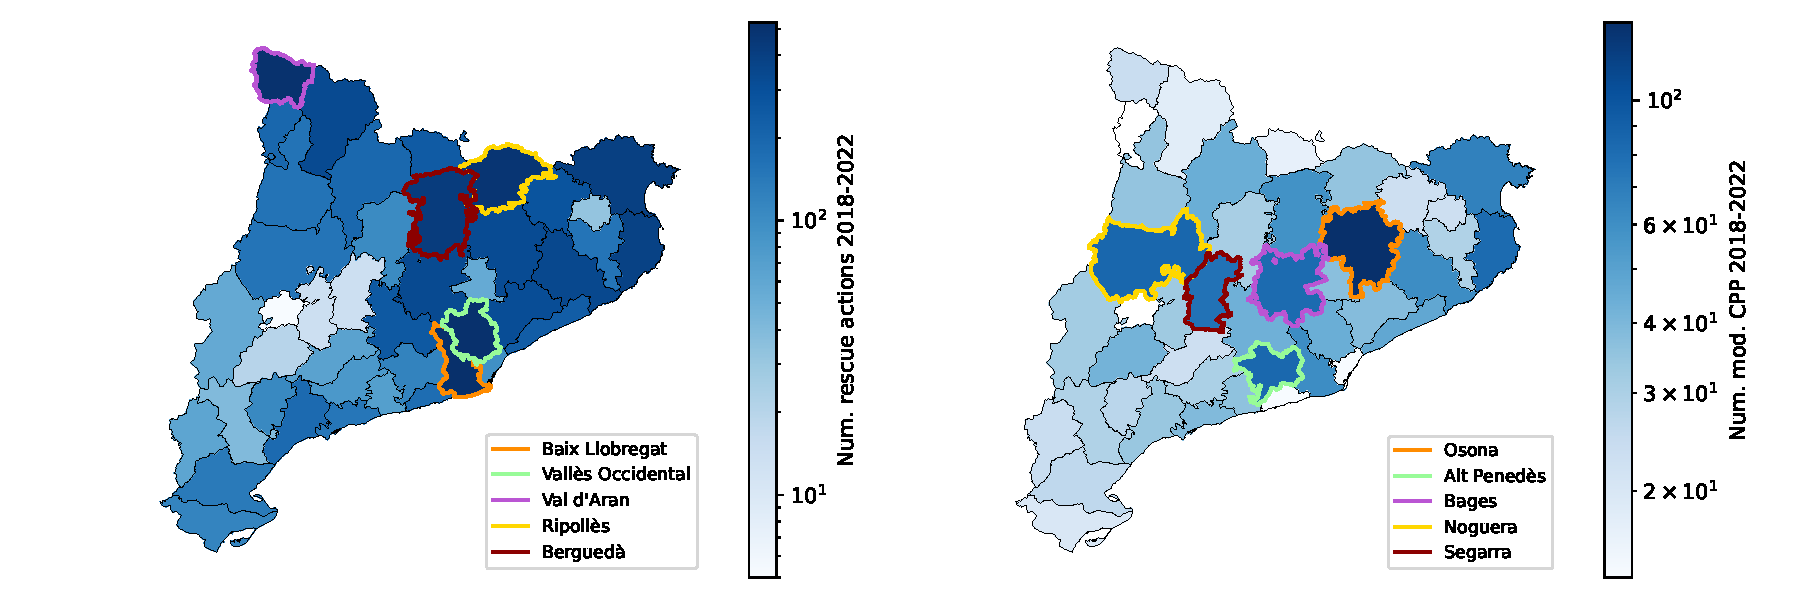
\includegraphics[width=1\linewidth]{../figures/merged_maps_plot}
\caption{Heatmaps showing the total number of rescue actions and modifications in CPP. In the left, we display the geographical plot generated for the total number of rescue actions. In the right, we display plot for the total count of changes in CPP. In both, we have highlighted the counties with most counts presented in the previous table Tab. \ref{tab:tab1}.}
\label{fig:fig1}
\end{figure}
From figure Fig. \ref{fig:fig1} we can observe that the counties with most rescue actions are, a priori, not geographically correlated with the counties which had most changes in CPP legal status. This can also be seen from the table Tab. \ref{tab:tab1}. We also note that there is a tendency of accumulating rescue actions towards the northern region of Catalonia, which could be caused by mountain rescue actions in the Pyrenees and pre-Pyrenees (this could be an extension to our project but we will not be entering into details) that have nothing to do with CPP but more of individual rescue actions. We also note that both Osona and Baix Llobregat have qualitatively different behaviours: Baix Llobregat is the county with most rescue actions but has rather a mild number of changes in CPP legal status, whilst Osona has a huge number of changes in CPP and also a great number of rescue actions. We then studied both counties separately by year, and found the results in figures Fig. \ref{fig:sub1}-\ref{fig:sub2}.

\begin{figure}
\centering
\begin{subfigure}{0.47\textwidth}
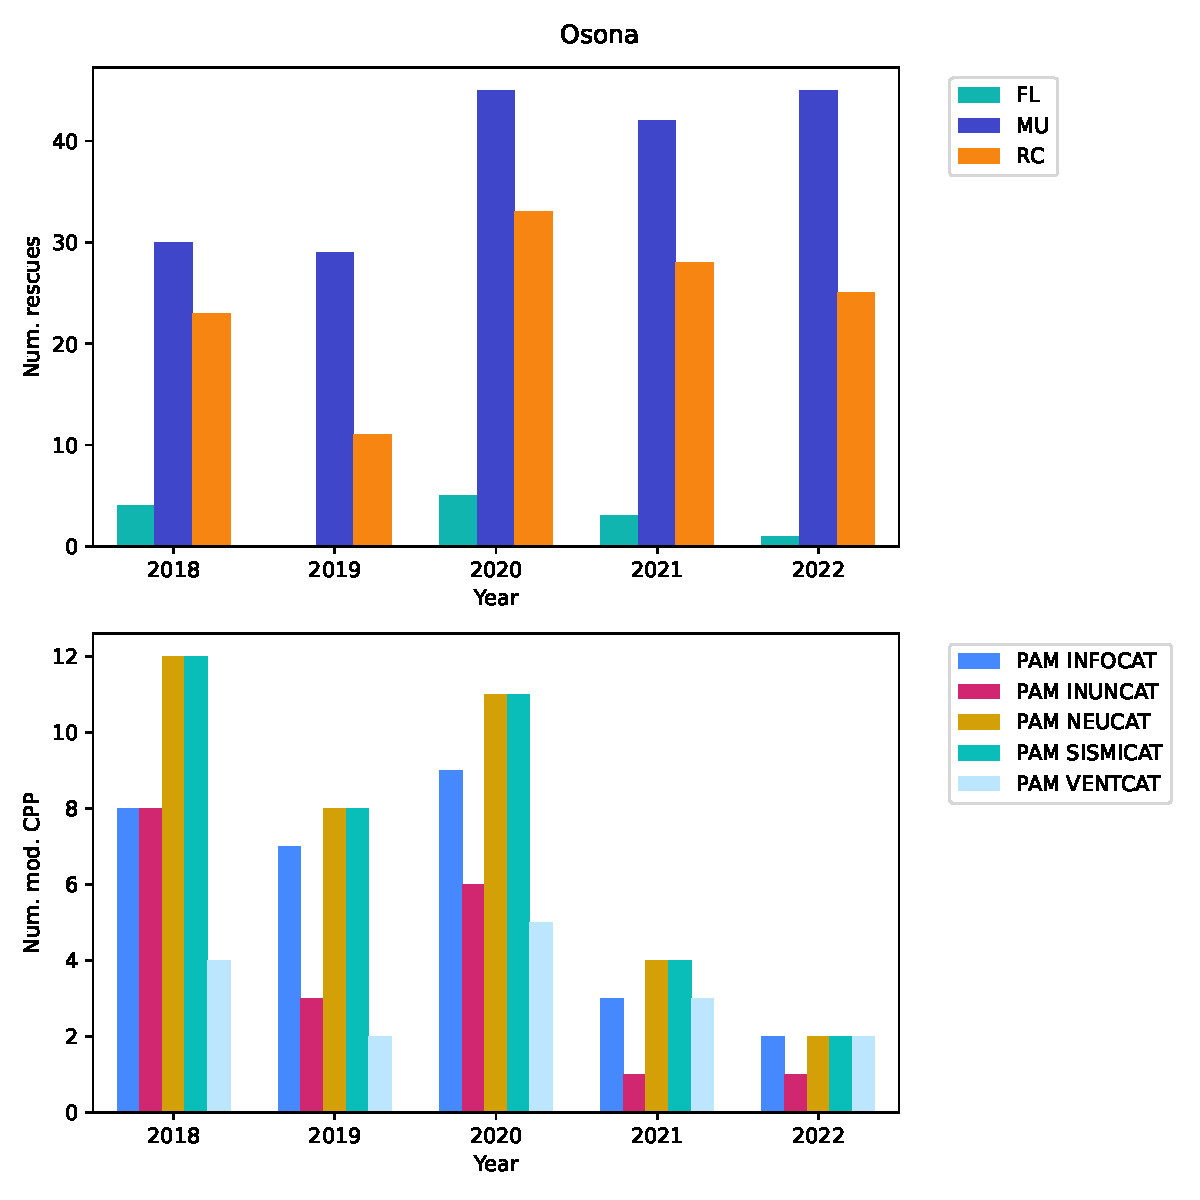
\includegraphics[width=\textwidth]{../figures/combined_plot_osona.pdf}
\caption{}
\label{fig:sub1}
\end{subfigure}\hskip1ex
\begin{subfigure}{0.47\textwidth}
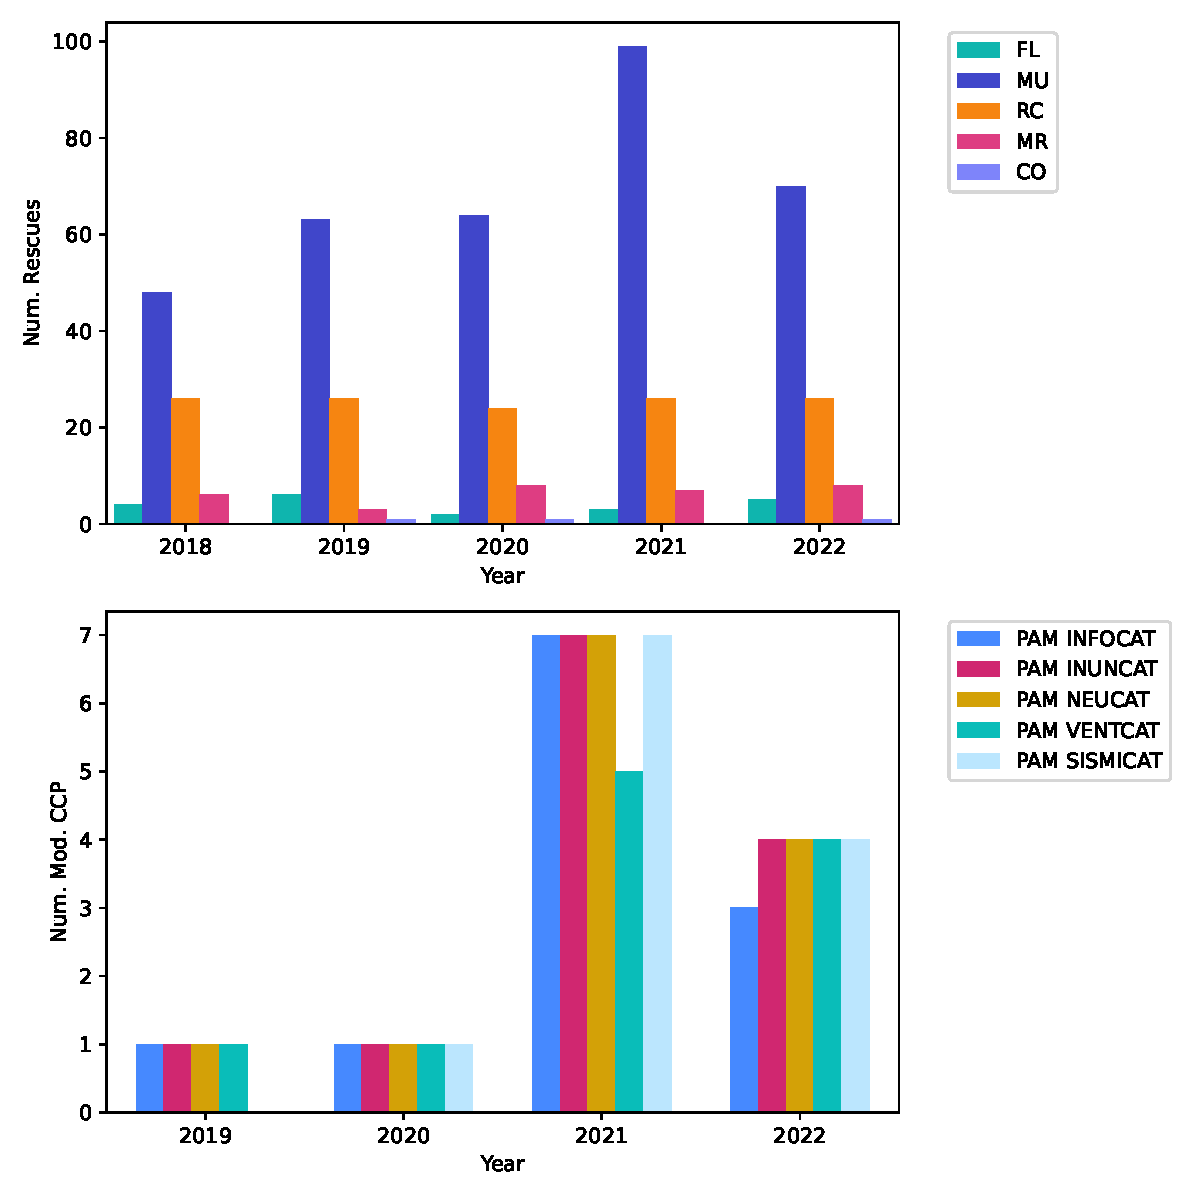
\includegraphics[width=\textwidth]{../figures/combined_plot_baix_llobregat.pdf}
\caption{}
\label{fig:sub2}
\end{subfigure}
\caption{Barplot showing the total count of rescue actions and changes in legal status of CPP per year hued by rescue and CPP typology. Subplot (a) correspond to data for Osona whilst subplot (b) corresponds to data for Baix Llobregat. For Baix Llobregat, no data was provided in the year 2018. Codes for rescue actions FL, MU, RC, MR and CO correspond to fluvial, mountain, research, maritime and cave rescues, respectively. Codes for CPP belong to different types of CPP.}
\end{figure}
As mentioned and without going into much detail, we can see that there is an evident different qualitative baviour: for Osona rescue actions seem to be somehow uncorrelated since peaks in changes of legal status of CPP do not match with rescue actions, whilst in the case of Baix Llobregat there is a well defined peak both in rescue actions and changes in CPP in the year 2021.

\section{Conclusions / Discussion}\label{sec:conclusions}
One of the main conclusions from the previous study is that, a priori, the rescue actions and the changes in legal status of CPP are uncorrelated at large time scale analysis. In most cases, rescue actions may be carried out in invidual and particular emergencies and mostly not in global civil threats or major civil protection actions. There can be, though, short time correlations between the previous in some cases, just as we have seen in the case of Baix Llobregat. 

The geographical heatmap on rescue actions by county also shows that there is an evident tendency of concentration of rescue action towards the northern region of Catalonia; which are actually related to the mountain enviroment rescue actions as our coleague Imma Passaret shows in their respective analysis of the data. The heatmap on changes in legal status of CPP suggest that these rescue actions are not related to civil protection.

Short-time correlations between rescue actions and modifcations of legal status of CPP put into test and evaluate the response of the public organisms towards global threats. Thus, in order to be able to make a thorough evaluation of the response of public organisms for civil protection we would need to improve date resolution of data, into probably date and time resolution. Future research could be carried along these matters of more thoroughly testing and evaluating the response of public organisms on civil protection.



\bibliographystyle{acm}
\bibliography{bibliography}

\end{document}